\section{Vision}\label{vision}

The vision of UxAS is to become the Government standard for verifiable
autonomy of multi-vehicle cooperative systems.

\section{Purpose/Goals}\label{purposegoals}

The purpose of UxAS is to enable unmanned vehicle (UxV) autonomy by
developing both a library of automated behaviors and the architecture to
connect them. The goals are to develop services and tasks that enhance
UxV autonomy, provide evidence of correct and safe system behavior, and
to demonstrate modularity and rapid integration of capabilities.

\section{Notional block diagram}\label{notional-block-diagram}

\begin{figure}
\centering
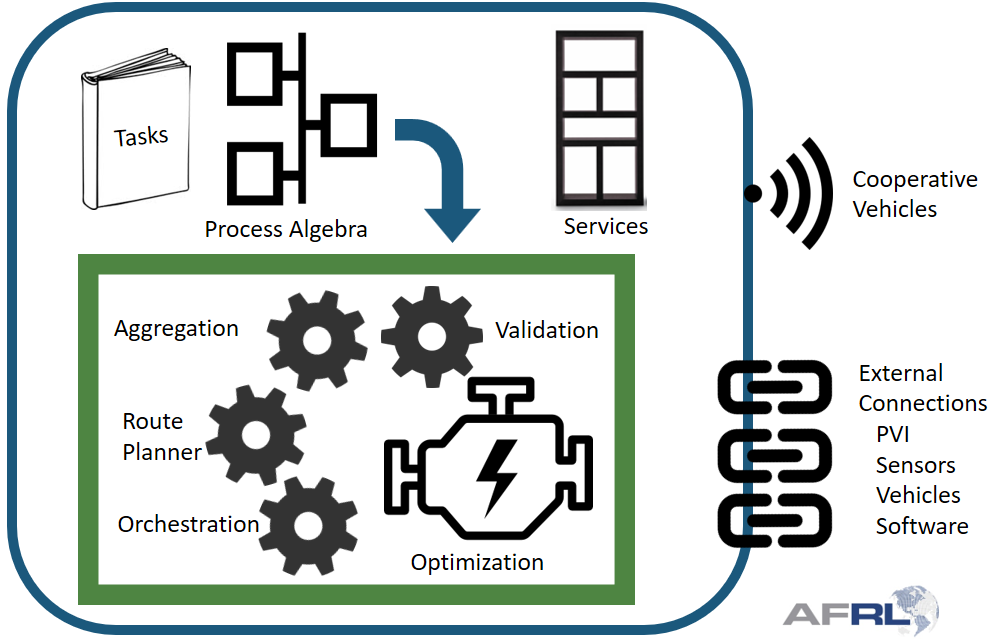
\includegraphics[width=0.4\textheight]{\FiguresPath//NotionalBlockDiagram.png}
\caption{Notional Block Diagram}
\end{figure}

\section{Feature list}\label{feature-list}

\section{Unmanned Systems Autonomy
Services}\label{unmanned-systems-autonomy-services}

UxAS is a software architecture that provides a framework to construct
and deploy software services that are used to enable autonomous
capabilities on-board unmanned systems. Along with the services, UxAS
provides a means for defining, implementing, and exchanging inter/intra
service messages. Based on many years of design, implementation, and
flight testing of collaborative algorithms for UAVs, UxAS was designed,
implemented, and flight tested for AFRL's ICE-T program. UxAS relies on
two software systems to provide services, the Lightweight Message
Construction Protocol (LMCP), and ZeroMQ.

LMCP was constructed by researchers at AFRL to provide a `structure for
common structured data and a process for serializing objects based on
those types' and `a method for encapsulating objects for transmission
between applications'{[}@Duquette:2010{]}. The ability for LMCP to use
Message Data Modules (MDM) makes it possible to define custom set of
messages for each target system. An example MDM is the Common Mission
Automation Services Interface (CMASI) which was designed to define data
relevant to mission planning and UAV autonomy.

UxAS uses ZeroMQ to implement intra-process, inter-process, vehicle to
vehicle, and vehicle to ground messaging. The authors describe ZeroMQ
this way: `looks like an embeddable networking library but acts like a
concurrency framework'{[}@ZeroMQBook:2013{]}. Inside each UxAS process
ZeroMQ publish/subscribe and push/pull nodes are used to implement a
data bus that is accessible to every in-process service. The services
are configured to subscribe to the LMCP messages that they require and
push any generated LMCP messages to the data bus.

UxAS is implemented in C++ and has been used with various operating
systems including, LINUX, Windows, OS X, and embedded LINUX. Services
inherit capabilities from a parent class that implements the core
functionality, i.e.~messaging, configuration, and execution. UxAS has
been used for applications such as implementing collaboration algorithms
onboard UAVs as well as implementing the core functionality of Unmanned
Ground Sensors (UGS) with communication links to the UAVs.
